\section{phpLogCon}
\subsection{Installation}
Der hier beschriebene Installations-Guide bassiert auf der englischen Beschreibung von der Webseite \\
\url{http://www.linuxjournal.com/content/centralized-logging-web-interface}.
Ich habe der Installation einige Arbeitsschritte hinzugefügt und auch einige verändert. Die hier beschriebene Installation ist zudem so nur unter Ubuntu möglich. Während der Installation wird mehrmals ein Texteditor benötigt. Ich verwende hierzu den Vim Editor. Für die Installation folgenden Befehl ausführen.

\begin{lstlisting}
sudo apt-get install vim
\end{lstlisting}

Desweiteren wird noch das Ubuntu Tool tasksel benötigt.

\begin{lstlisting}
sudo apt-get install tasksel
\end{lstlisting}

\subsubsection{Einrichtung eines Webservers}

Der LogAnalyzer ist eine Webanwendung, daher wird ein PHP fähiger Webserver mit einer Datenbankanbindung benötigt. Bevor wir den LogAnalyzer installieren können benötigen wir daher noch einige andere Software:

\begin{itemize}
\item Zeitsynchronisierung
\item MySQL Datenbank
\item Appache Webserver
\item PHP 5.01 oder höher
\item PHP5-GD
\end{itemize}

Damit alle Log-Dateien auch in der richtigen Reihenfolge angezeigt werden, müssen alle Systeme zeitlich synchronisiert werden. Hierzu dienen Zeitserver. Für die Synchronisation müssen folgende Befehle ausgeführt werden:
\begin{lstlisting}
sudo echo "ntpdate ntp.ubuntu.com" > /etc/cron.daily/ntpdate
sudo /etc/cron.daily/ntpdate
\end{lstlisting}

\subsubsection{Installation des Webservers}
Im Terminal folgendes eingeben:

\begin{lstlisting}
tasksel
\end{lstlisting}

In tasksel wählen wir \textit{LAMP Server} aus und bestätigen mit OK. Es folgt nun einen Installationsroutine in der einige Eingaben gemacht werden. Unter anderem wird dort, dass Passwort für die MySQL-Datenbank festgelegt. Dieses Passwort wird im weiteren Installationsverlauf noch benötigt. Nach Beendigung der Installation wird ein Neustart des Apache Servers empfohlen.

\begin{informationnote}
	Es ist zu empfehlen das System neu zu starten. 	Auf diese Weise wird sichergestellt, dass auch wirklich alle Dienste korrekt neu gestartet werden.
\end{informationnote}

\subsubsection{Einrichtung von rsyslog}
Die bisherige rsyslog Konfiguration muss für die Datenbank Anbindung erweitert werden. Zudem installieren wir noch ein Protokoll was später die Übertragungsgeschwindigkeiten deutlich verbessern wird. Zunächst werden folgende Pakete benötigt.

\begin{lstlisting}
sudo apt-get install rsyslog-mysql rsyslog-relp
\end{lstlisting}

Während der Installation gibt es die Möglichkeit die benötigte Tabellenstruktur anzulegen. Dieser Schritt ist zu empfehlen. Des weiteren wird man nach dem MySQL Passwort gefragt, welches man bei der vorigen Installation angeben musste. Um die Installation abzuschließen muss das rsyslog Passwort festgelegt werden. Die benötigte Konfiguration für rsyslog wurde im Kapitel 9.3 Remote Logging Konfiguration vorgenommen.

Zur Überprüfung ob die Log-Dateien wirklich in die Datenbank eingetragen werden, kann dieser Befehl verwendet werden. Dadurch wird die gesamte Tabelle der SystemEvents im Terminal ausgegeben.

\begin{lstlisting}
sudo mysql -p -e \"SELECT * FROM Syslog.SystemEvents;\"
\end{lstlisting}

\subsubsection{RELP}
RELP(\textbf{R}eliable \textbf{E}vent \textbf{L}ogging \textbf{P}rotocol) dient als Übertragungsprotokoll für Event-Logging und ist deutlich schneller als eine gewöhnliche UDP oder TCP Verbindung. Um das RELP zu aktivieren muss in \textit{/etc/rsyslog.conf} noch eine Anpassung vorgenommen werden.

In diese Datei muss folgendes einfügt werden:

\begin{lstlisting}
\$ModLoad imrelp
\$InputRELPServerRun 20514
\end{lstlisting}

\subsubsection{Hinzufügen eines Zwischenspeichers}
Um hohe Log-Datenmengen in die Datenbank problemlos aufnehmen zu können, empfiehlt es sich, einen Zwischenspeicher (Buffer) anzulegen. 
\begin{lstlisting}
sudo mkdir /var/rsyslog/work
\end{lstlisting}

Damit der Zwischenspeicher auch genutzt wird, muss noch folgendes zu \textit{/etc/rsyslog.conf} hinzugefügt werden.

\begin{lstlisting}
\$WorkDirectory /var/rsyslog/work \# default location for work (spool) files
\$ActionQueueType LinkedList \# use asynchronous processing
\$ActionQueueFileName dbq    \# set file name, also enables disk mode
\$ActionResumeRetryCount -1  \# infinite retries on insert failure
\end{lstlisting}

\begin{importantnote}
	Rsyslog muss nach dieser Änderung neu gestartet werden. Dies erfolgt mit \textit{/etc/init.d/rsyslog restart}. Administrationsrechte sind hierzu erforderlich.
\end{importantnote}

\subsubsection{LogAnalyzer}
Nachdem rsyslog richtig konfiguriert ist und die Log-Daten in der Datenbank gespeichert werden, muss der eigentliche Loganalyzer installiert und konfiguriert werden. Als erstes muss die aktuelle Version herunterladen werden.

\begin{lstlisting}
wget http://download.adiscon.com/loganalyzer/loganalyzer-3.2.1.tar.gz
\end{lstlisting}

Es empfiehlt sich immer die aktuelle stabile Version zu verwenden. Unter \url{http://loganalyzer.adiscon.com/downloads} kann in Erfahrung gebracht werden, welche Version aktuell ist. 
Die folgenden Schritte entpacken den Loganalyzer und übertragen die Dateien in den Apache Webserver.

\begin{informationnote}
	Zu beachten ist, das die Versionsnummer bei den Befehlen angepasst werden muss.
\end{informationnote}

\begin{lstlisting}
sudo tar -xzf loganalyzer-3.2.1.tar.gz 
cd loganalyzer-3.2.1
~/loganalyzer-3.2.1\# mkdir /var/www/logs
~/loganalyzer-3.2.1\# cp -R src/* /var/www/logs/
~/loganalyzer-3.2.1\# cp contrib/* /var/www/logs/
~/loganalyzer-3.2.1\# cd /var/www/logs/
/var/www/logs\#sudo  chmod +x configure.sh secure.sh
/var/www/logs\#sudo  ./configure.sh
\end{lstlisting}

Um die Benutzerverwaltung von Loganalyzer nutzen zu können, wird noch eine Datenbankstruktur benötigt.

\begin{lstlisting}
/var/www/logs\# mysql -p
mysql> create database LogAnalyzerUsers;
mysql> show databases;
mysql> grant all on LogAnalyzerUsers.* to LAUser@'localhost' identified by 'password';
mysql> quit
\end{lstlisting}

Für die letzten Konfigurationen nutzen Sie das Webinterface unter \url{http://myserver.tld/logs}. Hier können Sie einige Einstellungen vornehmen. Jede dieser Einstellungen können sie später auch über das Administratormenü korrigieren. 
Während der Konfiguration werden Sie aufgefordert, die Benutzerdatenbank anzugeben. Hierfür nutzen Sie die zuvor angelegte Datenbank LogAnalyzerUsers.
Danach müssen Sie die Grundeinstellungen der rsyslog Datenbank vornehmen. Die Standard Werte zeigen, dass es auch möglich wäre ohne eine Datenbank zu arbeiten. Dies ist jedoch bei einer hohen Anzahl von Systemen sehr langsam. Zudem wäre es nicht möglich beliebig viele Systeme in eine Analyse zu vereinen.

\begin{lstlisting}
Name                = vergeben Sie einen aussagekraeftigen Namen
Source Type         = MYSQL Native
Select View         = Syslog Fields
Table type          = MonitorWare
Database Host       = localhost
Database Name       = Syslog
Database Tablename  = SystemEvents
Database User       = root
Enable Row Counting = no
\end{lstlisting}

Danach sind die Einstellungen abgeschlossen. Wenn unter dem Menüpunkt \textit{Statistiken} die Diagramme nicht angezeigt werden, müssen Sie noch folgendes nachinstallieren.

\begin{lstlisting}
\$ sudo apt-get install php5-gd
\end{lstlisting}

Dies dient zur Darstellung von Graphiken unter PHP.

\subsection{Überblick und Möglichkeiten}
LogAnalyzer ist eine webbasierte Anwendung zur grafischen Darstellung von Log-Daten. Alle Daten werden in einer MySQL Datenbank gespeichert und über einen Apache Webserver grafisch dargestellt.

\subsubsection{Die Weboberfläche}
Die Weboberfläche ist in zwei Teile aufgeteilt. Im oberen Bereich befindet sich das Menü, in dem sämtliche Einstellungs- und Darstellungsmöglichkeiten zur Auswahl stehen.
Der untere Teil stellt den Wertebereich dar. In diesem wird je nach Auswahl entweder die Log-Tabelle oder die Statistik-Diagramme angezeigt.

\begin{figure}[h]
\begin{center}
 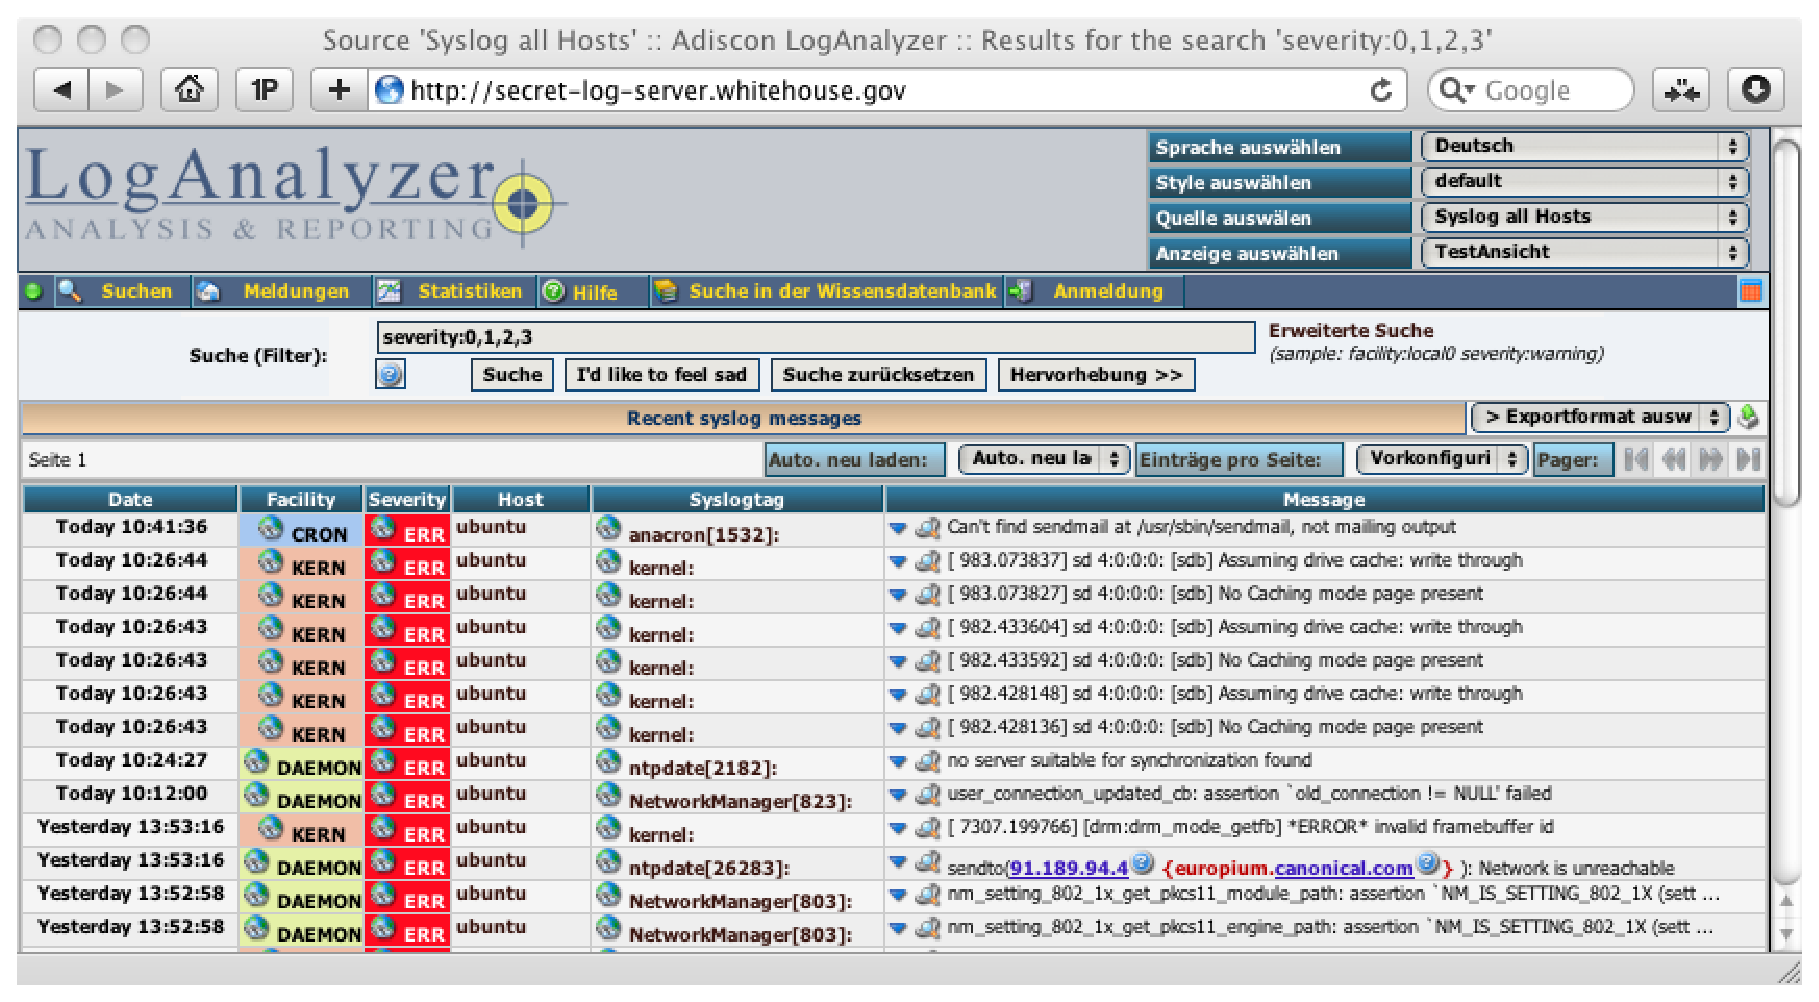
\includegraphics[width=\textwidth]{content/images/loganalyzer.eps}
  \caption{Screenshot Webinterface LogAnalyzer}
\end{center}
\end{figure}

\subsubsection{Das Menü}
\subsubsection*{Suche}
Mit Hilfe der Suche lassen sich viele verschiedene Auswahlkriterien treffen. Sie bietet nicht nur die Möglichkeit Schlüsselwörtern zu verwenden, sondern auch nach diversen Auswahlkriterien zu Filtern.
\begin{itemize}
\item Zeitliche Abgrenzung
\item Syslog Meldungen
\item Syslog Kategorie Filter
\item Syslog Dringlichkeit Filter
\item Meldung Typ
\item Syslogtag
\item Quelle (Hostname)
\end{itemize}

Diese Suchfunktion ermöglicht es große Mengen an Log-Daten einfach und effizient zu Filtern. Damit können aussagekräftige Darstellungen schnell erzeugt werden.

\subsubsection*{Meldungen}
Unter Meldungen findet man alle gespeicherten Log-Daten, zeitlich sortiert. Die Darstellung ist eine Tabelle in der folgende Informationen enthalten sind:
\begin{itemize}
\item DATE: Zeitpunkt des Logs
\item FACILITY: Anlage
\item SERVERITY:  Sicherheitseinstufung
\item HOST: von wem ist die Meldung
\item SYSLOGTAG
\item PROZESSID
\item MASSAGETYP
\item MELDUNG: die eigentliche Meldung des Logs
\end{itemize}

Weiterhin gibt es eine Schnellsuchfunktion, in der ein einfacher Filter oder ein Suchwort eingegeben werden kann. Für die Schnellsuchfunktion kann man auch Filter vordefinieren, die über ein Auswahlmenü erreichbar sind. Genaueres hierzu finden sie unter Administration.
%TODO: LINK!

\subsubsection*{Statistiken}
Hier werden statistische Auswertungen mit Hilfe von Diagrammen dargestellt. Welche das genau sind bleiben dem Anwender überlassen. Unter dem Menüpunkt Administration (Login erforderlich) gibt es das Untermenü Charts. Dort können beliebige Diagramme erstellt werden.
Genauere Informationen: siehe Administration
%TODO: LINK!

\subsubsection*{Administration}
Im \textit{Administrationsmenü} können sämtliche Einstellungen vorgenommen werden. Unter anderem:
\begin{itemize}
\item Grundeinstellung korrigieren
\item neue Quellen können hinzugefügt 
\item verwendete Felder in Meldungen bearbeiten 
\item Anzeigearten festgelegt
\item Diagramme erstellen
\item Meldungs Parser 
\item Report Modules 
\item DB Manager
\item Benutzerverwaltung
\item Gruppenverwaltung
\end{itemize}

Unter Quellen ist es möglich weitere Verbindungen anzugeben oder Bestehende zu verändern. Als Quellen können nicht nur MySQL-Datenbanken verwendet werden, sondern auch einzelne Log-Dateien oder andere Datenbanken (PDO).

Der Menüpunkt Suchen bietet die Möglichkeit Filterfunktionen für das Hauptmenü zu definieren. Hierbei ist es möglich Suchfunktionen für bestimmte Gruppen oder Benutzer festzulegen.

Es gibt drei Arten von Diagrammen. Horizontales Balkendiagramm, vertikales Balkendiagramm und Kuchendiagramm. Welcher Inhalt genau dargestellt werden soll, wird nach der gleichen Syntax, wie in den Filterfunktionen angegeben.

Weitere Informationen zur Diagrammerstellung kann auf der Internetseite von LogAnalyzer nachgelesen werden \url{http://loganalyzer.adiscon.com/doc/manual.html}.